% --------------------------------------------------------------------------
% Template for DMRN 2021 paper; to be used with:
%          dmrn2021.sty  - DMRN 2021 LaTeX style file
% Adapted from dcase2016.sty
% --------------------------------------------------------------------------

\documentclass{article}
\usepackage{caption}
\usepackage{times,amsmath,graphicx,url,dmrn2020}
\usepackage{indentfirst}
\setlength{\parskip}{0.5em}

% smaller font size for captions
\captionsetup[figure]{font=footnotesize,labelfont=footnotesize}
\captionsetup[table]{font=footnotesize,labelfont=footnotesize}

% reduce blank space after figures
\setlength{\belowcaptionskip}{-10pt}

% Example definitions.
% --------------------
\def\defeqn{\stackrel{\triangle}{=}}
\newcommand{\symmat}[1]{{\mbox{\boldmath $#1$}}}

% roman numbering of sections
\renewcommand{\thesection}{\Roman{section}} 

% Title.
% --------------------
\title{Building style-aware neural MIDI synthesizers using simplified differential DSP approach}

% Single addresses (uncomment and modify for single-address case).
% --------------------
% \oneauthor
% {Given-name Family-name(Surname)\sthanks{Research supported by ABC Foundation.}}
% {Department/Research Institute, University, Country}
% {john@fictional.edu}

% Two addresses
% --------------------
\twoauthors
 {Sergey Grechin}
    {Infinite Album}
    {grechin.sergey@gmail.com}
 {Given-name Family-name (Surname)}
    {Department/Research Institute, University, Country}
    
\begin{document}
%\ninept
\tenpt
\maketitle

\begin{sloppy}
\begin{abstract}
We explore how simplified differential DSP approach can be used to build realistically sounding virtual MIDI-controllable synthesizers. The simplification involves directly using  MIDI data as input to the DDSP decoder. On top of that, we show how  incorporating additional style-based and temporal channels can be used to imitate various aspects of performance and improve realism.  We further demonstrate the results of applying the approach to the task of modelling the sound of electric guitar. The presented results were obtained with a model trained on less than 12 minutes of manually MIDI-annotated audio. The source code is released along with the prepared dataset.
\end{abstract}

\begin{keywords}
Deep Learning, DDSP, virtual synthesizers, MIDI
\end{keywords}

\section{Headings}
\label{sec:headings}
This template provides authors with most of the formatting specifications needed for preparing electronic versions of their papers. A brief abstract (containing text only) must also be entered in the above ``Abstract'' headed text box.

Headings may be used as required. Please adopt the Small-Caps heading style. References and figures may be included if necessary. But the overall paper cannot exceed the one page limit. Do not change the margins, column widths, font sizes or line spacing to squeeze more text into the page. Use \textit{italics} for emphasis; do not underline. 

\section{Others}
\label{sec:others}
Define abbreviations and acronyms the first time they are used in the text, even after they have been defined in the abstract. Do not use abbreviations in the title or heads unless they are unavoidable. Use either SI (MKS) or CGS as primary units (SI units are encouraged).

%You will need to determine whether or not your equation should be typed using either the Times New Roman or the Symbol font (please no other font). To create multileveled equations, it may be necessary to treat the equation as a graphic.%
Equation numbers, within parentheses, are to position flush right, as in (1). Italicize Roman symbols for quantities and variables, but not Greek symbols. Use a long dash rather than a hyphen for a minus sign. Be sure that the symbols in your equation have been defined before or immediately following the equation.

Use the caption package to declare smaller font sizes for figure and table labels. Use words rather than symbols or abbreviations when writing Figure axis labels to avoid confusing the reader. If including units in the label, present them within parentheses. Do not label axes only with units. In the example, write “Magnetization (A/m)”, not just “A/m”. Do not label axes with a ratio of quantities and units. For example, write “Temperature (K)”, not “Temperature/K.”


\begin{figure}[t]
  \centering
  \centerline{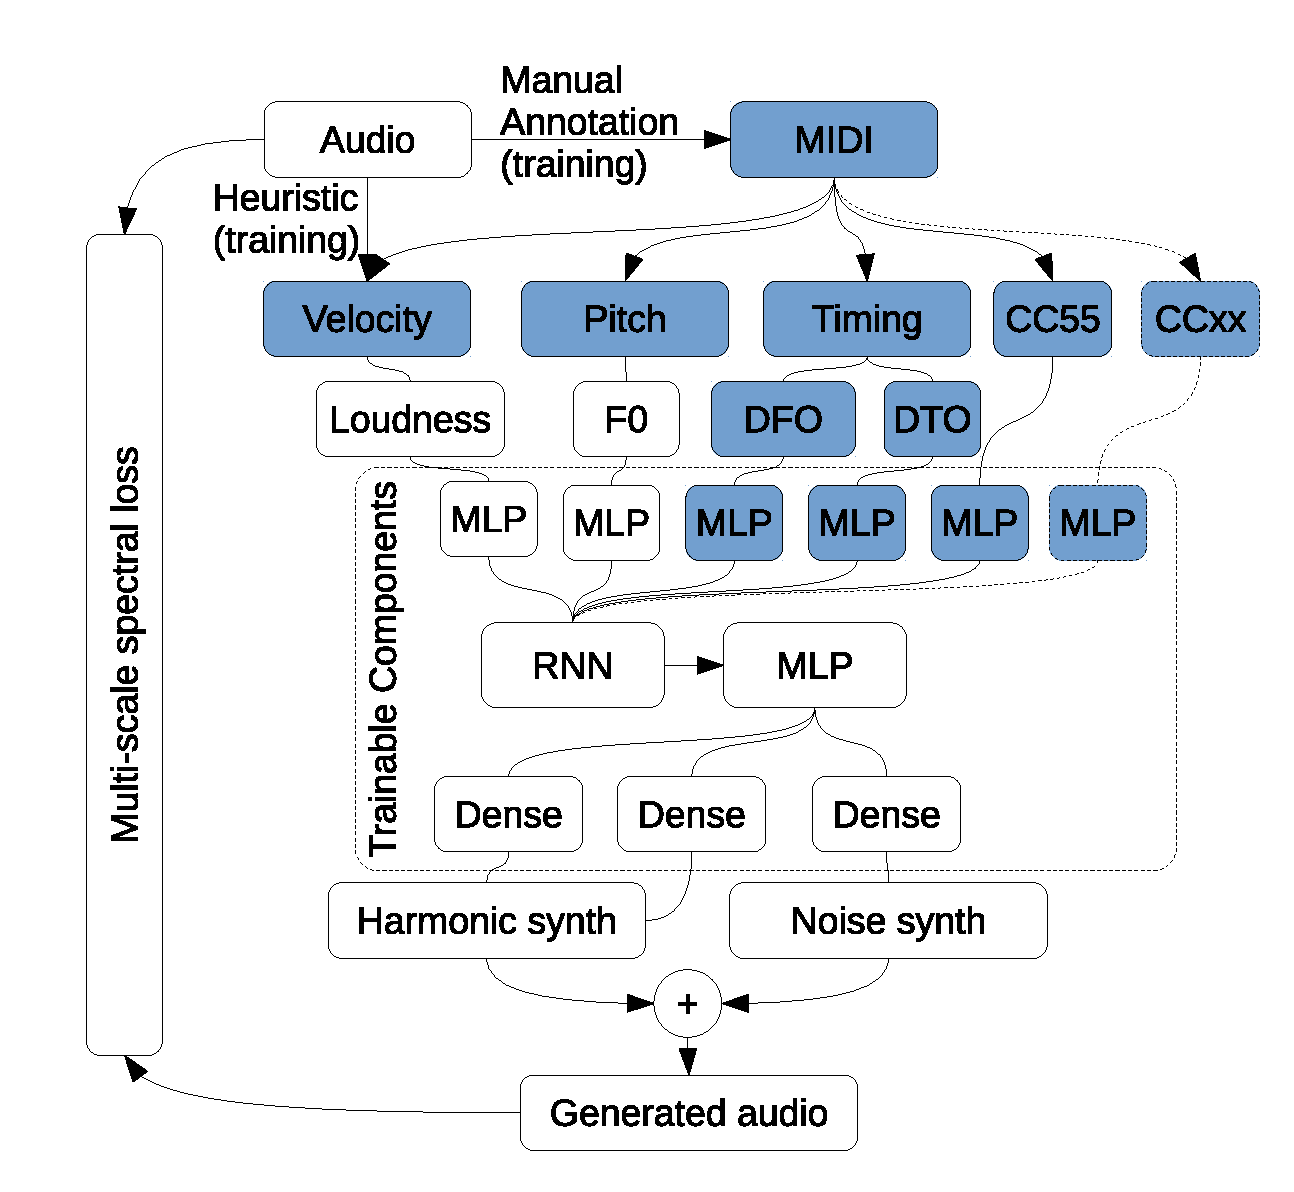
\includegraphics[scale=0.4]{components}}
  \caption{Componenets of the model. The unfilled blocks represent the original DDSP design. 
MLP - Multilayer perceptron, 
DFO - distance from onset, 
DTO - distance to offset,
CC - continuous controller
}
  \label{fig:components}
\end{figure}

\begin{figure}[t]
  \centering
  \centerline{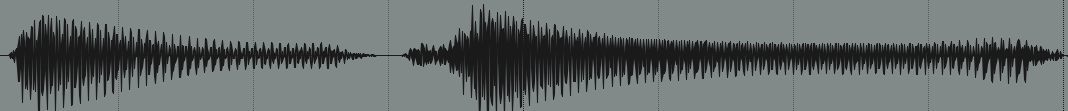
\includegraphics[scale=0.32]{generated_waveform}}
  \caption{Waveforms generated on C-5 for two MIDI notes with closed and open sound.}
  \label{fig:generated_waveform}
\end{figure}



List and number \cite{IEEEPDFSpec} all bibliographical references at the end of the paper. The references should be numbered in order of appearance in the document. When referring to them in the text, type the corresponding reference number in square brackets as shown at the end of this sentence .

The preferred spelling of ``acknowledgment'' is without an “e” after the “g”. Avoid ``One of us (R. B. G.) thanks''; try ``R. B. G. thanks''. Put sponsor acknowledgments in the footnote.



% 
% ------------------------------------------------------------
% Either list references using the bibliography style file IEEEtran.bst

\bibliographystyle{IEEEtran}
{\footnotesize\bibliography{refs}}

% \bibliography{refs}

\end{sloppy}
\end{document}
